\actTitle{2.2 - Introduction to Polynomial Functions}

\noindent \textbf{Topics:}  polynomials, leading term test, intermediate value theorem\\

\noindent \textbf{Student Learning Outcomes:}
\begin{enumerate}
\item Students will be able to determine the end behavior of a polynomial function.
\item Students will be able to identify zeros and multiplicities of zeros.
\item Students will be able apply the Intermediate Value Theorem.

\end{enumerate}

\hrule 

\bigskip

\subsection{End Behavior of Polynomial Functions} ~

\begin{boxthm}
{\bf Definition of a Polynomial Function}
Let $n$ be a positive, whole number and $a_n,a_{n-1}, a_{n-2}...,a_1,a_0$ be real numbers, where $a_n\neq 0$.  Then a function defined by $$f(x)=a_nx^n+a_{n-1}x^{n-1}+a_{n-2}x^{n-2}+...+a_1x+a_0$$ is called a \textbf{polynomial function of degree $n$}.

\end{boxthm}


Examples:
$$f(x)=5x^2+8x^4 \quad \quad \quad g(x)=\frac{x^2+3}{x^2} \quad \quad \quad  h(x)=4x^5-3x^4+2x^2 \quad \quad \quad k(x)=4\sqrt{x}-\frac{3}{x} +x^2$$

\vfill
We have already studied several special cases of polynomial functions:

$$f(x)=2 \quad \quad \quad g(x)=3x+1 \quad \quad \quad  h(x)=4x^2+7x-1$$


\vfill

Polynomial functions of degree 2 or higher have graphs that are smooth and continuous.\\[.5in]


\clearpage



\subsection{The Leading Coefficient Test}

As $x$ gets very large (more positive) or very small (more negative),
the graph of the polynomial function
\begin{eqnarray}
  \label{eq:2-2:generalPoly}
  f(x) & = & a_n x^n + a_{n-1} x^{n-1} + a_{n-2} x^{n-2} + \cdots +
             a_1 x + a_0, ~~(a_n \neq 0),
\end{eqnarray}
either rises or falls. The long term behaviour depends on whether or
not $n$ is even or odd, and it also depends on whether or not the
value of $a_n$ is positive or negative. There are four possibilities.

First, if $n$ is an odd number, then the long term behaviour is
different when comparing very large values of $x$ to very small values
of $x$.

      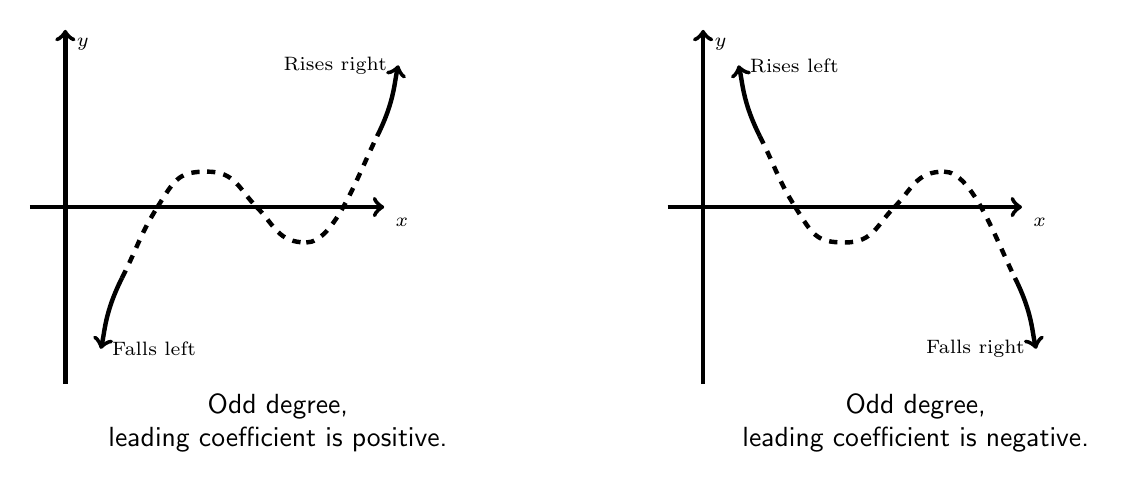
\begin{tikzpicture}[y=0.9cm, x=0.9cm,font=\sffamily]
        \begin{scope} %[shift={(0,8)}]
           \draw[ultra thick,->] (-0.5,0) -- coordinate (x axis mid) (4.5,0)
                node[font=\scriptsize,anchor = north west] {$x$}; 
           \draw[ultra thick,->] (0,-2.5) -- coordinate (y axis mid) (0,2.5) 
                node[font=\scriptsize,anchor = west,shift={(0.0,-0.2)}]  {$y$};

           \draw[ultra thick,black,<-]
           (0.5,-2) .. controls +( 0.06,0.24) and +(-0.25, -0.5) .. (0.8,-1)
               node[font=\scriptsize,anchor=west,pos=0] {Falls left};
           \draw[ultra thick,black,->]
           ( 4.4,1) .. controls +( 0.25, 0.5) and +(-0.06,-0.24) .. (4.7,2)
           node[font=\scriptsize,anchor=east,pos=1] {Rises right};

           \draw[ultra thick,black,dashed]
              (0.8,-1)  .. controls +( 0.25, 0.5)  and +(-0.25,-0.4) .. (1.3,0)
              (1.3,0)   .. controls +( 0.25, 0.4)  and +(-0.4,0.0)   .. (2,0.5)
              (2,0.5)   .. controls +( 0.4, 0.0)   and +(-0.25, 0.25) .. (2.7,0)
              (2.7,0)   .. controls +( 0.25,-0.25) and +(-0.4,0.0)   .. (3.4,-.5)
              (3.4,-.5) .. controls +( 0.4, 0.0)  and +(-0.25,-0.5)  .. (4.4,1)
              ;

           \node[black,anchor=north,shift={(0,0)},align=center] at (3,-2.5)
              {Odd degree, \\ leading coefficient is positive.};

        \end{scope}

        \begin{scope}[shift={(9,0)}]
           \draw[ultra thick,->] (-0.5,0) -- coordinate (x axis mid) (4.5,0)
                node[font=\scriptsize,anchor = north west] {$x$}; 
           \draw[ultra thick,->] (0,-2.5) -- coordinate (y axis mid) (0,2.5) 
                node[font=\scriptsize,anchor = west,shift={(0.0,-0.2)}]  {$y$};

           \draw[ultra thick,black,<-]
           (0.5,2) .. controls +( 0.06,-0.24) and +(-0.25, 0.5) .. (0.8,1)
               node[font=\scriptsize,anchor=west,pos=0] {Rises left};
           \draw[ultra thick,black,->]
           ( 4.4,-1) .. controls +( 0.25, -0.5) and +(-0.06,0.24) .. (4.7,-2)
           node[font=\scriptsize,anchor=east,pos=1] {Falls right};

           \draw[ultra thick,black,dashed]
              (0.8,1)  .. controls +( 0.25, -0.5)  and +(-0.25,0.4) .. (1.3,0)
              (1.3,0)   .. controls +( 0.25,-0.4)  and +(-0.4,0.0)   .. (2,-0.5)
              (2,-0.5)   .. controls +( 0.4, 0.0)   and +(-0.25, -0.25) .. (2.7,0)
              (2.7,0)   .. controls +( 0.25,0.25) and +(-0.4,0.0)   .. (3.4,.5)
              (3.4,.5) .. controls +( 0.4, 0.0)  and +(-0.25,0.5)  .. (4.4,-1)
              ;

           \node[black,anchor=north,shift={(0,0)},align=center] at (3,-2.5)
              {Odd degree, \\ leading coefficient is negative.};

        \end{scope}

      \end{tikzpicture}

Secondly, if $n$ is an even number, then the long term behaviour
is the same when comparing very large values of $x$ to very
small values of $x$.


      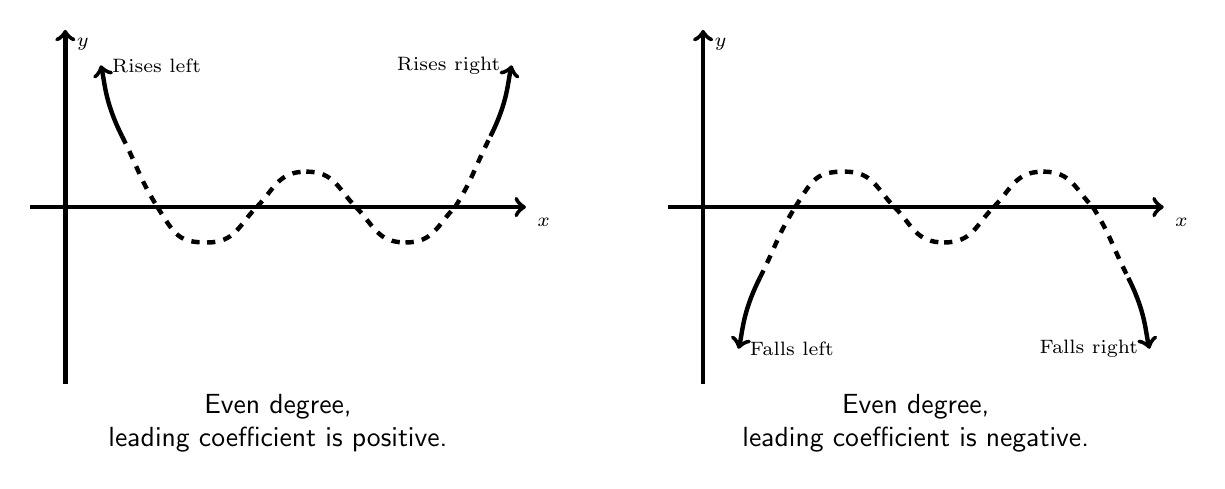
\begin{tikzpicture}[y=0.9cm, x=0.9cm,font=\sffamily]
        \begin{scope} %[shift={(9,0)}]
           \draw[ultra thick,->] (-0.5,0) -- coordinate (x axis mid) (6.5,0)
                node[font=\scriptsize,anchor = north west] {$x$}; 
           \draw[ultra thick,->] (0,-2.5) -- coordinate (y axis mid) (0,2.5) 
                node[font=\scriptsize,anchor = west,shift={(0.0,-0.2)}]  {$y$};

           \draw[ultra thick,black,<-]
           (0.5,2) .. controls +( 0.06,-0.24) and +(-0.25, 0.5) .. (0.8,1)
               node[font=\scriptsize,anchor=west,pos=0] {Rises left};
           \draw[ultra thick,black,->]
           ( 6.0,1) .. controls +( 0.25,0.5) and +(-0.06,-0.24) .. (6.3,2)
           node[font=\scriptsize,anchor=east,pos=1] {Rises right};

           \draw[ultra thick,black,dashed]
              (0.8,1)  .. controls +( 0.25, -0.5)  and +(-0.25,0.4) .. (1.3,0)
              (1.3,0)   .. controls +( 0.25,-0.4)  and +(-0.4,0.0)   .. (2,-0.5)
              (2,-0.5)   .. controls +( 0.4, 0.0)  and +(-0.25, -0.25) .. (2.7,0)
              (2.7,0)   .. controls +( 0.25,0.25)  and +(-0.4,0.0)   .. (3.4,.5)
              (3.4,.5) .. controls +( 0.4, 0.0)    and +(-0.25,0.25)  .. (4.1,0.0)
              (4.1, 0.0) .. controls +(0.25,-0.25) and +(-0.4,0.0) .. (4.8,-0.5)
              (4.8,-0.5) .. controls +(0.4,0.0)    and +(-0.25,-0.25) .. (5.5,0.0)
              (5.5, 0.0) .. controls +(0.25,0.4)   and +(-0.25,-0.5)   .. (6.0,1.0)
              ;

           \node[black,anchor=north,shift={(0,0)},align=center] at (3,-2.5)
              {Even degree, \\ leading coefficient is positive.};

        \end{scope}

        \begin{scope}[shift={(9,0)}]
           \draw[ultra thick,->] (-0.5,0) -- coordinate (x axis mid) (6.5,0)
                node[font=\scriptsize,anchor = north west] {$x$}; 
           \draw[ultra thick,->] (0,-2.5) -- coordinate (y axis mid) (0,2.5) 
                node[font=\scriptsize,anchor = west,shift={(0.0,-0.2)}]  {$y$};

           \draw[ultra thick,black,<-]
           (0.5,-2) .. controls +( 0.06,0.24) and +(-0.25,-0.5) .. (0.8,-1)
               node[font=\scriptsize,anchor=west,pos=0] {Falls left};
           \draw[ultra thick,black,->]
           ( 6.0,-1) .. controls +( 0.25,-0.5) and +(-0.06,0.24) .. (6.3,-2)
           node[font=\scriptsize,anchor=east,pos=1] {Falls right};

           \draw[ultra thick,black,dashed]
              (0.8,-1)  .. controls +( 0.25, 0.5)  and +(-0.25,-0.4) .. (1.3,0)
              (1.3,0)   .. controls +( 0.25, 0.4)  and +(-0.4,0.0)   .. (2,0.5)
              (2,0.5)   .. controls +( 0.4, 0.0)  and +(-0.25, 0.25) .. (2.7,0)
              (2.7,0)   .. controls +( 0.25,-0.25)  and +(-0.4,0.0)   .. (3.4,-.5)
              (3.4,-.5) .. controls +( 0.4, 0.0)    and +(-0.25,-0.25)  .. (4.1,0.0)
              (4.1, 0.0) .. controls +(0.25,0.25) and +(-0.4,0.0) .. (4.8,0.5)
              (4.8, 0.5) .. controls +(0.4,0.0)    and +(-0.25,0.25) .. (5.5,0.0)
              (5.5, 0.0) .. controls +(0.25,-0.4)   and +(-0.25,0.5)   .. (6.0,-1.0)
              ;

           \node[black,anchor=north,shift={(0,0)},align=center] at (3,-2.5)
              {Even degree, \\ leading coefficient is negative.};

        \end{scope}

      \end{tikzpicture}


\clearpage

\begin{enumerate}

\item Use the leading term test to determine the function's end behavior.


\begin{enumerate}
\item $f(x)=-7x^5+2x^3+7x+5$
\vfill

\item $f(x)=\frac{1}{4}x(2x-3)^3(x+4)^2$
\vfill

\end{enumerate}

\subsection{Identify Zeros and Multiplicities of Zeros} ~

\begin{boxthm}
{\bf Multiplicities and $x$-Intercepts}
If $f$ is a polynomial function, then the values of $x$ for which $f(x)=0$ are called the \textbf{zeros (roots or solutions)} of $f(x)$.  Each real root of the polynomial equations appears as an $x$-intercept of the graph of the polynomial function.\\
\\
If $r$ is a zero of \textbf{even multiplicity}, then the graph \textbf{touches} the $x$-axis and \textbf{turns around} at $r$.  If $r$ is a zero of \textbf{odd multiplicity}, then the graph \textbf{crosses} the $x$-axis at $r$.  Regardless of whether the multiplicity of a zero is even or odd graphs tend to flatten out near zeros with multiplicity greater than one.
\end{boxthm}




\item Find the zeros for each polynomial function and give the multiplicity for each.  State whether the graph crosses the $x$-axis, or touches the $x$-axis and turns around, at each zero.

\begin{enumerate}
\item $f(x)=4(x+3)(x-7)^2$
\vfill
\item $f(x)=x^3-6x^2+9x$
\vfill
\end{enumerate}


\newpage

\subsection{Apply the Intermediate Value Theorem} ~

\begin{boxthm}
{\bf Intermediate Value Theorem}
Let $f$ be a polynomial function.  For $a<b$, if $f(a)$ and $f(b)$ have opposite signs, then $f$ has at least one zero on the interval $[a,b]$.
\end{boxthm}

\item Use the Intermediate Value Theorem to determine if $f(x)=4x^4-8x^2+2$ has a real zero on the interval $[-1,0]$.
\vfill


\item Sketch a graph of $f(x)=x^3-9x$
\vfill
\vfill
\vfill



\end{enumerate}

\noindent \textbf{Student Learning Outcomes Check}

\begin{enumerate}
\item Are you able to determine the end behavior of a polynomial function?
\item Can you identify zeros and multiplicities of zeros?
\item Are you able apply the Intermediate Value Theorem?
\end{enumerate}

\noindent \textbf{If any of your answers were no, please ask about these topics in class.}

